\documentclass{article}

\title{A Short Introduction to Coxme}
\author{Terry Therneau \\
        Mayo Clinic}
% \VignetteIndexEntry{Introduction}
\usepackage{Sweave}
\begin{document}
\maketitle

\section{Introduction}
 The \texttt{coxme} function fits mixed-effects Cox models of the following
form
\begin{eqnarray}
  \lambda(t) &=& \lambda_0(t) e^{X\beta + Z b} \label{eq1} \\
  b &\sim & N(0, \Sigma) \nonumber
\end{eqnarray}
where \begin{itemize}
  \item $\lambda(t)$ is the hazard function
  \item $\lambda_0(t)$ is an unspecified baseline hazard
  \item $\beta$ is the vector of fixed effects, with design matrix $X$
  \item $b$ is the vector of random effects, with design matrix $Z$,
    which are drawn from a Gaussian distribution with variance $\Sigma$
\end{itemize}

The first version of the code was distributed as a part of the \texttt{kinship}
package in R, in recognition of the fact that it was primarily targeted
towards genetic problems.  It was also distributed as part of the base
survival package in S-Plus.  The current version is more broad in its
capabilities, and is also designed for ready extension.

\section{Simple random effects}
Let us start with a very simple model.  
Mantel \cite{Mantel} gives a data example of a carcinogen experiment
using 150 rats, 3 each from 50 litters.  One rat from each
litter was injected with a powerful carcinogen, and the time
to tumor development recorded. The following fits a 
random intercept per litter  to the data in addition to the
treatment effect.
\begin{Schunk}
\begin{Sinput}
> library(coxme)
> fit1 <- coxme(Surv(time, status) ~ rx + (1 | litter), data = rats)
> print(fit1)
\end{Sinput}
\begin{Soutput}
Cox mixed-effects model fit by maximum likelihood
  Data: rats
  events, n = 40, 150
  Iterations= 10 54 
                    NULL Integrated Penalized
Log-likelihood -185.6556   -180.849 -173.7754

                  Chisq    df         p   AIC    BIC
Integrated loglik  9.61  2.00 0.0081757  5.61   2.24
 Penalized loglik 23.76 13.16 0.0356550 -2.57 -24.80

Model:  Surv(time, status) ~ rx + (1 | litter) 
Fixed coefficients
        coef exp(coef)  se(coef)    z      p
rx 0.9132666  2.492451 0.3226843 2.83 0.0047

Random effects
 Group  Variable  Std Dev   Variance 
 litter Intercept 0.6522673 0.4254526
\end{Soutput}
\end{Schunk}

The printed output contains
\begin{itemize}
  \item The information portion. This shows the data set, the total number
    of observations (150) and the total number of events, and the number
    of iterations for the overall maximization (solving for $\Sigma$) and
    the subsidiary ones maximizing over $b$ and $\beta$.  Last is the
    log partial likelihood for the null model, the value for the full
    model with $b$ integrated out, and the full model's value without
    integration.
  \item The chisquare statistics for the model, viewed from two perspectives.
    \begin{itemize}
      \item A traditional random-effects perspective, i.e., with the
        random effects $b$ integrated out.  From this perspective there are
        two parameters, one for the fixed treatment \texttt{rx} effect, and one for
        the variance of the random effect.
      \item A penalized likelihood approach, where the random effects have not
        been integrated out. 
    \end{itemize}
  \item The estimated values for the fixed effects.  Treatment has a
    large effect, increasing the hazard almost 2.5 fold.
  \item The estimated values for the random effects.  The random intercept terms
    $b$ for each litter have variance $\Sigma = \sigma^2 I$, with
    $\hat\sigma = $ 0.65
\end{itemize}

The integrated partial likelihood (IPL) and penalized partial likelihood (PPL)
are two different views on the same fit.  The IPL takes the more traditional
random effects approach, whereas the PPL is closely related to smoothing
splines and generalized additive models.  Neither is more 'correct' than the
other and both provide a useful perspective; asymptotics for the IPL p-values
are more thoroughly worked out, however.  
From the PPL perspective, we have fit a model that is intermediate between one
that had no litter effect, and one that had entered litter as a factor; the
former would have 0 degrees of freedom for litter and the latter 49 degrees
of freedom; this fit used 12.16 df for litter and 1 for treatment.

The astute reader has noticed by now that there is no printed estimate for
the standard error of the variance $\hat\sigma^2$.  This is on purpose,
primarily because the profile likelihood function for $\sigma$ is 
highly asymmetric and thus any confidence intervals based on it would be
dubious at best.  
The overall significance of the random effect can be tested by comparing it
to the results for a fixed-effects model.
\begin{Schunk}
\begin{Sinput}
> fit0 <- coxph(Surv(time, status) ~ rx, rats)
> print(fit0)
\end{Sinput}
\begin{Soutput}
Call:
coxph(formula = Surv(time, status) ~ rx, data = rats)


    coef exp(coef) se(coef)    z      p
rx 0.905      2.47    0.318 2.85 0.0044

Likelihood ratio test=7.98  on 1 df, p=0.00474  n= 150 
\end{Soutput}
\end{Schunk}
The formal test compares the partial likelihood LRT for a model with
$\sigma^2=0$, i.e., the fixed effects model with the IPL for the
fitted random effects model, giving a value of 9.61 - 7.98 = 1.63 on
(2-1) = 1 degree of freedom.

Another way to look at the effect is to draw the profile likelihood,
which we compute below for first the fixed effect and then the  random effect.
The number of points (30) was arbitrary; enough to produce a smooth curve.
\begin{Schunk}
\begin{Sinput}
> profile.x <- matrix(0, nrow = 30, ncol = 2)
> profile.y <- profile.x
> profile.x[, 1] <- seq(0.25, 1.6, length = 30)
> profile.x[, 2] <- seq(0.05, 2, length = 30)
> for (i in 1:30) {
+     tfit <- coxme(Surv(time, status) ~ offset(rx * profile.x[i, 
+         1]) + (1 | litter), data = rats)
+     profile.y[i, 1] <- tfit$loglik[2]
+     tfit <- coxme(Surv(time, status) ~ rx + (1 | litter), data = rats, 
+         vfixed = profile.x[i, 2])
+     profile.y[i, 2] <- tfit$loglik[2]
+ }
> matplot(profile.x, 2 * (profile.y - fit0$loglik[1]), xlab = "Parameter estimate", 
+     ylab = "Profile likelihood", type = "l", lty = 1, col = 1:2)
> abline(h = 2 * diff(fit1$loglik)[1] - qchisq(0.95, 1), lty = 2)
> legend(1.5, 9, c("Fixed", "Random"), lty = 1, col = 1:2)
\end{Sinput}
\end{Schunk}
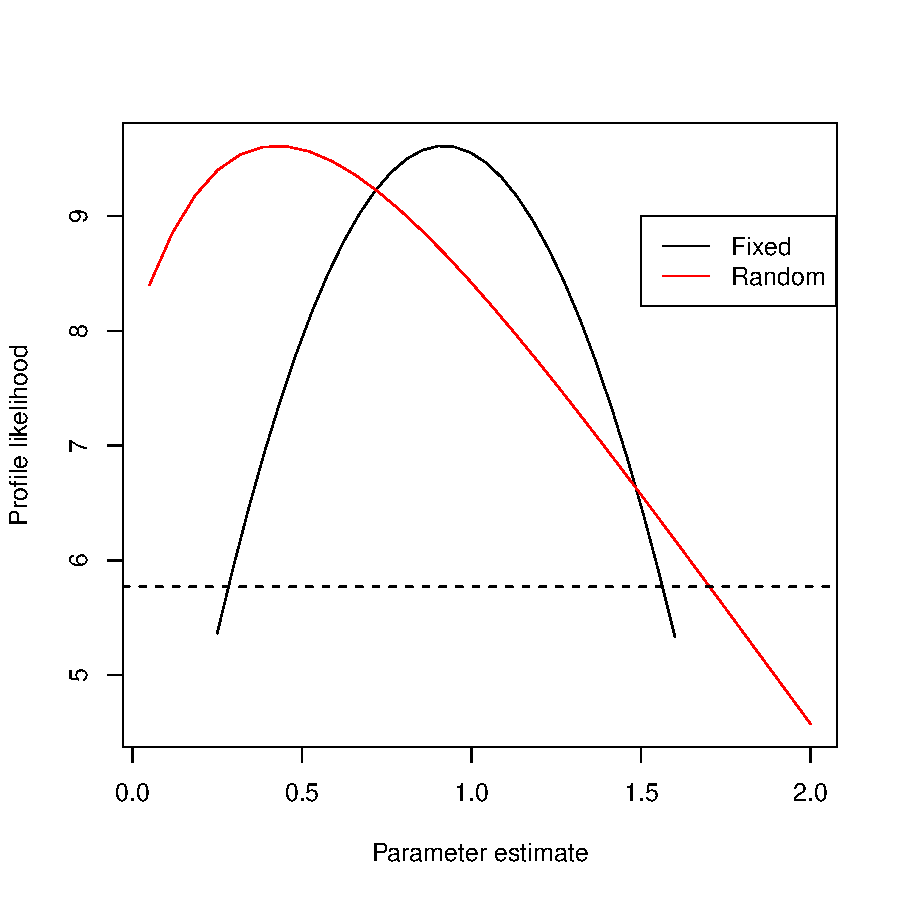
\includegraphics{intro-003}

I have plotted twice the difference between the IPL and the null fit in order to
put the plot on a familiar chisqare scale. (Note that \texttt{fit1} and \texttt{fit0} have
the same logliklihood for their ``null'' or baseline models.)
A horizontal line has been drawn 3.84 units down from the maximum value,
the profile based confidence interval is the intersection of the 
curves with this line.  The CI for $\sigma^2$ clearly includes zero.

\section{Random treatment effect}
The \texttt{eortc} data set is a simulation, but based on an actual European
Oncology Research Trail Consortium study.  The data set has 37 centers
with enrollment ranging from 21 to 247 in each center, and was created to
understand the ability of random effects with respect to center and
treatment by center differences \cite{cortinas}.
Models for treatment with and without a center effect are
\begin{Schunk}
\begin{Sinput}
> efit0 <- coxph(Surv(y, uncens) ~ trt, eortc)
> efit1 <- coxme(Surv(y, uncens) ~ trt + (1 | center), data = eortc)
> efit2 <- coxme(Surv(y, uncens) ~ trt + (1 | center) + (trt | 
+     center), data = eortc)
> efit3 <- coxme(Surv(y, uncens) ~ trt + (1 + trt | center), eortc)
> 2 * (c(efit0$loglik[2], efit1$loglik[2], efit2$loglik[2], efit3$loglik[2]) - 
+     efit0$loglik[1])
\end{Sinput}
\begin{Soutput}
           Integrated Integrated Integrated 
  105.6578   236.1108   246.1194   247.1241 
\end{Soutput}
\end{Schunk}
In this case the improvement is significant as we go from a simple
treatment model to one with random intercepts per center,
random intercept and slope, and correlated intercept and slope.

As can be seen from above, a coxme model can have multiple
random effects.
\begin{itemize}
  \item A random effect is any term in parenthesis that contains
    a vertical bar, with a grouping variable on the right and 
    covariates on the left.  An intercept term is never
    assumed, e.g. (trt | center) has only a treatment effect.
  \item The grouping effect can be nested, as in (1| school/teacher)
    for random school and teacher within school effects.
  \item By defaut, a full covariance matrix is assumed.  Model 2
    shows that a simple way to specify independence is to
    place the effects in separate terms.
\end{itemize}

\section{Shrinkage}
Coefficient shrinkage can also be placed in the context of a mixed
effects model.  
The lung cancer data set contains survival information on a set of subjects
with advanced disease, in a study that was designed to assess the
importance of various patient factors on prognosis.  One of the
stonger variables is \texttt{ph.ecog}, the physician's assessment of
the ECOG performace score.  This is a variable that goes from 0 (no physical
restrictions) to 3 for severe disability with respect to activities of
daily living such as meal preparation, bathing, etc.
Below are two simple models treating the score as continuous or as
a categorical.
\begin{Schunk}
\begin{Sinput}
> coxph(Surv(time, status) ~ ph.ecog, lung)
\end{Sinput}
\begin{Soutput}
Call:
coxph(formula = Surv(time, status) ~ ph.ecog, data = lung)


         coef exp(coef) se(coef)   z       p
ph.ecog 0.476      1.61    0.113 4.2 2.7e-05

Likelihood ratio test=17.6  on 1 df, p=2.77e-05  n=227 (1 observation deleted due to missingness)
\end{Soutput}
\begin{Sinput}
> coxph(Surv(time, status) ~ factor(ph.ecog), lung)
\end{Sinput}
\begin{Soutput}
Call:
coxph(formula = Surv(time, status) ~ factor(ph.ecog), data = lung)


                  coef exp(coef) se(coef)    z       p
factor(ph.ecog)1 0.369      1.45    0.199 1.86 6.3e-02
factor(ph.ecog)2 0.916      2.50    0.225 4.08 4.5e-05
factor(ph.ecog)3 2.208      9.10    1.026 2.15 3.1e-02

Likelihood ratio test=18.4  on 3 df, p=0.000356  n=227 (1 observation deleted due to missingness)
\end{Soutput}
\end{Schunk}
 The first model estimates an increase of .48 per category, the second has
increments of .37, .55, and 1.29.  
One concern with the second model is that the final coefficient depends on
very few subjects, only 1 in fact, and so is unstable.
A shrinkage model may be more suitable:
\begin{Schunk}
\begin{Sinput}
> ecog0 <- 1 * (lung$ph.ecog == 0)
> ecog1 <- 1 * (lung$ph.ecog == 1)
> ecog2 <- 1 * (lung$ph.ecog == 2)
> ecog3 <- 1 * (lung$ph.ecog == 3)
> sfit <- coxme(Surv(time, status) ~ (ecog0 + ecog1 + ecog2 + ecog3 | 
+     1), lung)
> print(sfit, rcoef = TRUE)
\end{Sinput}
\begin{Soutput}
Cox mixed-effects model fit by maximum likelihood
  Data: lung
  events, n = 164, 227 (1 observation deleted due to missingness)
  Iterations= 19 99 
                    NULL Integrated Penalized
Log-likelihood -744.4805  -739.4681 -737.0748

                  Chisq   df          p   AIC  BIC
Integrated loglik 10.02 1.00 0.00154450  8.02 4.92
 Penalized loglik 14.81 1.86 0.00050178 11.09 5.32

Model:  Surv(time, status) ~ (ecog0 + ecog1 + ecog2 + ecog3 | 1) 
Penalized coefficients
              coef exp(coef) Penalized se
1.ecog0 -0.4265719 0.6527429    0.2792069
1.ecog1 -0.1098388 0.8959786    0.2721517
1.ecog2  0.3831532 1.4669027    0.2782519
1.ecog3  0.1532575 1.1656251    0.4326039

Random effects
 Group Variable    Std Dev   Variance 
 1     (Shrinkage) 0.4413178 0.1947614
\end{Soutput}
\end{Schunk}
By default the printout from a coxme model does not include the 
estimates of the random coefficients $b$.
(In many cases there will be several hundred of them.)
The \texttt{rcoef} argument overrides this.  In either case the
estimated values $\hat b$
can be found in the \texttt{frail} component of the returned fit.
For the shrunken fit the risk differences are .31, .49 and -.23; 
the risk for the ecog==3 group has been severly curtailed.

Unlike the standard choices for treatment contrasts ('contr.treatment', etc)
that select one of the levels as comparison group, and thus return $k-1$
coefficients for a factor with $k$ levels, the natural constraint for
random effects is a sum constraint: $k$ coefficients are returned that sum
to zero.  So in the above we created 4 dummy variables to represent all
four levels of the ECOG score.  
For automatically created coeffients $b$ such as in the EORTC example
above, you will find that the \texttt{fit\$frail} component likewise
has one element for each of the 37 institutions.

\end{document}
